\label{sec:methods}

\section{Meteorological forcing data}
% The research method by which you will investigate the world. 
% A short summary of the available methods
% Your choice
% Detailed report of how you actually carried out your research. 
% Presenting how you selected the people taking part is of special importance.


Forcing data are used to drive the hydrological model. Shyft needs precipitation, relative humidity, temperature, wind speed and incoming shortwave radiation as input data. \autoref{tab:datasets} gives a summary of the forcing data used in this study.


\begin{table}[ht]
    \centering
    \caption{Summary of the forcing datasets}
    \label{tab:datasets}
    \resizebox{\textwidth}{!}{%
    \begin{tabular}{llllll}
    \toprule
    \textbf{Forcing} & \textbf{Data} & \textbf{Spatial} & \textbf{Temporal} & \textbf{n} & \textbf{Reference} \\
    \textbf{dataset} & \textbf{period} & \textbf{resolution} & \textbf{resolution} &  & \\
    \hline
    WFDE5 & 1990-2019 & 0.5◦ × 0.5◦ & Hourly & 9 & \autocite{cucchiWFDE5BiasadjustedERA52020} \\
    ERA5 + TopoScale & 1999-2015 & 0.5◦ × 0.5◦ & Hourly & & \autocite{hersbachERA5HourlyData2018} \\
    \bottomrule         
    \end{tabular}%
    }
\end{table}




\subsection{Reanalysis and regional climate data}

\subsubsection{WFDE5}

The bias-adjusted ERA5 reanalysis data for impact studies (WFDE5) is generated through applying the WATCH Forcing Data methodology to surface meteorological variables from the ERA5 reanalysis \autocite{cucchiWFDE5BiasadjustedERA52020}. Reanalysis data is a combination of model data and worldwide observations into a globally complete and consistent dataset using the laws of physics \autocite{cucchiWFDE5BiasadjustedERA52020}. The WFDE5 dataset contains 11 variables with an hourly temporal resolution on a regular longitude-latitude 0.5 degree grid. The dataset has a global coverage, but is only defined at land and lake points. The WFDE5 dataset is spanning from January 1979 to the end of 2019, and has been adjusted using an elevation correction and monthly-scale bias based on Climatic Research Unit (CRU) data (for temperature, diurnal temperature range, cloud-cover, wet days number and precipitation fields). The datasets used for monthly bias-correction are CRU TS4.03 from CRU \autocite{harrisVersionCRUTS2020} from 1979 to 2019 for all variables, and the GPCCv2018 full data product \autocite{schneiderGPCCFullData2018} for rainfall. The dataset is distributed by the Copernicus Climate Change Service (C3S) through the Climate Data Store (CDS) as monthly netCDF files that are downloaded as zip-files or compressed tar files \autocite{copernicusclimatechangeserviceSurfaceMeteorologicalVariables2020}. NetCDF files are self-describing data that are machine-independent. The netCDF format supports creation, access, and sharing of array-oriented scientific data. The data can be downloaded via the CDS API or through the \href{https://cds.climate.copernicus.eu/cdsapp#!/dataset/reanalysis-era5-single-levels?tab=overview}{C3S Climate Data Store}.

\autoref{tab:wfde5_variables} shows the names and units of the near-surface variables from WFDE5 used in this study. 


% Please add the following required packages to your document preamble:
% \usepackage{graphicx}
% Please add the following required packages to your document preamble:
% \usepackage{graphicx}
\begin{table}[ht]
\centering
\caption{WFDE5 variables}
\label{tab:wfde5_variables}
\resizebox{\textwidth}{!}{%
\begin{tabular}{llll}
\toprule
\textbf{Variable name} & \textbf{Description} & \textbf{Units} & \textbf{\begin{tabular}[c]{@{}l@{}}Data for monthly \\ bias correction\end{tabular}} \\
\hline
Wind    & 10 m wind speed                    & m s$^{-1}$            & Nil  \\
Tair    & 2 m air temperature                & K                     & 1)   \\
PSurf   & Pressure at the surface            & Pa                    & Nil  \\
SWdown  & Downward shortwave radiation flux  & W m$^{-2}$            & 2)   \\
Rainf   & Rainfall flux                      & kg m$^{-2}$ s$^{-1}$  & 3)   \\
Snowf   & Snowfall flux                      & kg m$^{-2}$ s$^{-1}$  & 3)   \\
Qair    & 2 m specific humidity              & kg kg$^{-1}$          & Nil  \\

\bottomrule
\multicolumn{4}{l}{1) CRU TS4.03 temperature and diurnal temperature range} \\
\multicolumn{4}{l}{2) CRU TS4.03 cloud and effects of inter-annual changes in atmospheric loading}                                                     \\
\multicolumn{4}{l}{3) ERA5 ratio of rainfall/precipitation and snowfall gauge correction}                                                            
\end{tabular}%
}
\end{table}

 Shyft requires the units of the forcing data to be converted into standard input units. Temperature was converted from Kelvin (K) to Celsius degrees ($^{\circ}$C) by simply subtracting 273.15 from the absolute temperature. Similarly, the surface pressure was converted from Pa to hPa by multiplying with 0.01. Precipitation was converted to mm h$^{-1}$ by summing the snowfall flux (kg m$^{-2}$ s$^{-1}$) and the rainfall flux (g m$^{-2}$ s$^{-1}$), and then multiplying the sum with 3600 (s h$^{-1}$). 
 
The relative humidity was calculated using the MetPy package in Python \autocite{mayMetPyMeteorologicalPython2022}. The relative humidity function in this package calculates relative humidity from total atmospheric pressure (hPa), air temperature ($^{\circ}$C) and specific humidity (kg kg$^{-1}$). The formula is based upon \autocite{wallaceAtmosphericScienceIntroductory1977} and \autocite{salbyFundamentalsAtmosphericPhysics1996a}. 

The units of wind (m s$^{-1}$) and global radiation (W m$^{-2}$) were not converted. 

\begin{equation}
    RH = \frac{q}{(1 - q) w_{s}}
\end{equation}

where $RH$ is relative humidity as unitless ratio,  $q$ is the specific humidity and $w_{s}$ is the saturation mixing ratio. The saturation mixing ratio is the ratio between the density of water vapor and the density of dry air \autocite{kasaharaWeatherPredictionNumerical2003}. 


\subsubsection{ERA5}

The ERA5 dataset is the fifth generation reanalysis from the European Centre for Medium-Range Weather Forecasts (ECMWF) \autocite{hersbachERA5HourlyData2018}. The dataset provides hourly estimates for a large number of atmospheric, ocean-wave and surface quantities. The data is available from 1950 to present, and has been re-gridded to a regular lat-lon grid of 0.25 degrees. The dataset is updated daily, and can be downloaded in either GRIB or netCDF format from the CDS API or the \href{https://cds.climate.copernicus.eu/cdsapp#!/dataset/reanalysis-era5-single-levels?tab=overview}{C3S Climate Data Store}.

\section{Topographical Data}

The SRTM 1 Arc-Second Global elevation data from the NASA's Shuttle Radar Tomography Mission (NASA-SRTM) provides a worldwide coverage of void filled data filled with a resolution of 1 arc-second ($\sim$ 30 meters) \autocite{earthresourcesobservationandscienceeroscenterShuttleRadarTopography2017}. The Digital Elevation Model (DEM) data can be downloaded from the coverage map in the  \href{https://earthexplorer.usgs.gov/}{USGS Earth Explorer}. Each GeoTIFF file covers 1 degree tiles, and is about 25 MB each.

\autoref{tab:srtm} shows the DEM data that was downloaded for this study.

% Please add the following required packages to your document preamble:
% \usepackage[table,xcdraw]{xcolor}
% If you use beamer only pass "xcolor=table" option, i.e. \documentclass[xcolor=table]{beamer}
\begin{table}[ht]
\centering
\caption{SRTM 1 Arc-Second Global}
\label{tab:srtm}
\begin{tabular}{ll}
\toprule
Projection                        & Geographic                       \\
Horizontal datum                  & WGS84                            \\
Vertical Datum                    & EGM96 (Earth Gravitational Mode) \\
Vertical Units                    & Meters                           \\
Spatial resolution                & 1 Arc-second ($\sim$ 30 m)       \\
Raster size                       & 1 degree tiles                   \\
Tiles                             & N25-31 E82-88                    \\
C-band wavelength                 & 5.6 cm                           \\ 
\bottomrule
\end{tabular}
\end{table}

The DEM files were merged into one DEM file in QGIS. This DEM file was then opened in Python using the  \href{https://rasterio.readthedocs.io/en/latest/index.html}{Rasterio package} which reads and writes GeoTIFF files, and provides a Python API based upon Numpy N-dimensional arrays and GeoJSON. The coordinate points from the forcing data were then sampled in the DEM file to get the elevations needed for the Shyft input data.

\section{Land Cover Data Sets}

The Land Cover Classification System (LCCS) Land Cover Map Fine Resolution V2.3 Global dataset from the GlobCover Portal provides global composites and land cover maps \autocite{bontempsGLOBCOVER2009Products2011}. The GlobCover products have been processed by ESA and by the Université Catholique de Louvain using input observations from the 300 m MERIS sensor on board on the ENVISAT satellite mission. The land cover maps covers December 2004 - June 2006 and January - December 2009. The surface reflectance mosaic products are projected in a Platé-Carré projection (WGS84 ellipsoid) with a 1/360° pixel resolution. The land cover classes as defined by a set of classifiers. 

\section{Validation datasets}

\subsection{Observed river discharge} 

Daily stream flow data from the period 2000-2015 is obtained from The Department of Hydrology and Meteorology, DHM. The  flow gauging station is located at Arguhat bazaar (485 m.a.s.l) at 28.043611$^{\circ}$ N and 84.816389$^{\circ}$ E. The station has been operating since 28 November 1963. 

\subsection{Snow Products}

The High Mountain Asia (HMA) snow reanalysis data set from the NASA Snow and Ice Data Center (NSIDC) covers the period 1 October 1999 to 30 September 2017 with a daily temporal resolution and 16 arc-seconds x 16 arc-seconds spatial resolution \autocite{margulisHighMountainAsia2021}. 


\section{Pre-processing of data}

\subsection{TopoScale}

\subsection{Catchment Discretization Technique}


\section{Hydrological Modeling Framework}


Shyft is an open-source cross-platform hydrological toolbox built to provide a computation framework for spatially distributed hydrologic models \autocite{burkhartShyftV4Framework2021}. The platform is developed by Statkraft AS, the largest generator of renewable energy in Europe, in cooperation with the research community at the University of Oslo. The Shyft software is developed for operational, regional-scale hydropower inflow forecasting, and it aims to i$)$ provide a flexible forecasting toolbox for operational environments, ii$)$ facilitate computationally efficient calculations of hydrologic response at the regional scale, iii$)$ enable the use of multiple hypothesis to quantify forecast uncertainties, iv$)$ allow for multiple model forcing configurations, and v$)$ promote expeditious implementations of the findings from research into operational modeling. 

One of the strengths of Shyft is that multiple models may be built through the creation of hydrologic algorithms from a library of well known routines or by the construction of new routines \autocite{burkhartShyftV4Framework2021}. The user of Shyft can get access to all of the components of the framework via Python through an application programming interface (API), while still having high computational performance as the algorithms are implemented in modern C++. This API set-up enables rapid use of different model configurations and selection of an optimal forecast model. 

Since the Shyft toolbox is built for operational, region-scale hydropower inflow forecasting, some of its key design principles vary from what may be prioritized in a pure research environment \autocite{burkhartShyftV4Framework2021}. Shyft is well-documented open source code and follows the latest code standards, due to the strict requirements regarding software security, testing and code quality in an operational environment. One of the key concepts in the Shyft philosophy is that "data should live at the source". This implies that users of Shyft are encouraged to write their of repositories that connect directly to the source data. This is done to ensure that the data is always up-to-date and that the data is not stored in multiple places. Another key design principle of Shyft facilitates flexible entry points for novel algorithms, while also testing these in parallel with operational runs. This also allows for flexible and exploratory research.

\subsection{The architecture of Shyft}

The Shyft platform is distributed through three GitLab repositories: \href{https://gitlab.com/shyft-os/shyft}{shyft}, \href{https://gitlab.com/shyft-os/shyft-data}{shyft-data} and \href{https://gitlab.com/shyft-os/shyft-doc}{shyft-docs}. The shyft repository contains the source code for the Shyft platform, while the shyft-data repository contains the test-data needed for the full runs and demo. The shyft-docs repository contains the end-user documentation for the Shyft platform. Additionally, there is also a \href{https://gitlab.com/shyft-os/dockers}{Dockers} repository that contains the Docker build recipes for the Shyft eco-system.

The Shyft platform is built on top of C++ and Python \autocite{burkhartShyftV4Framework2021}. Basic data structures, hydrologic algorithms and models in the Shyft core is written in C++ to provide high computational efficiency \autocite{zehraComparativeAnalysisPython2020}. The C++ code is then compiled into a Python extension module, which is then imported into Python. The Shyft API which is coded in Python is the main interface for the user to interact with the Shyft platform.  \autoref{fig:shyft_architecture} shows the architecture of the Shyft platform. 

\begin{figure}[ht]
    \centering
    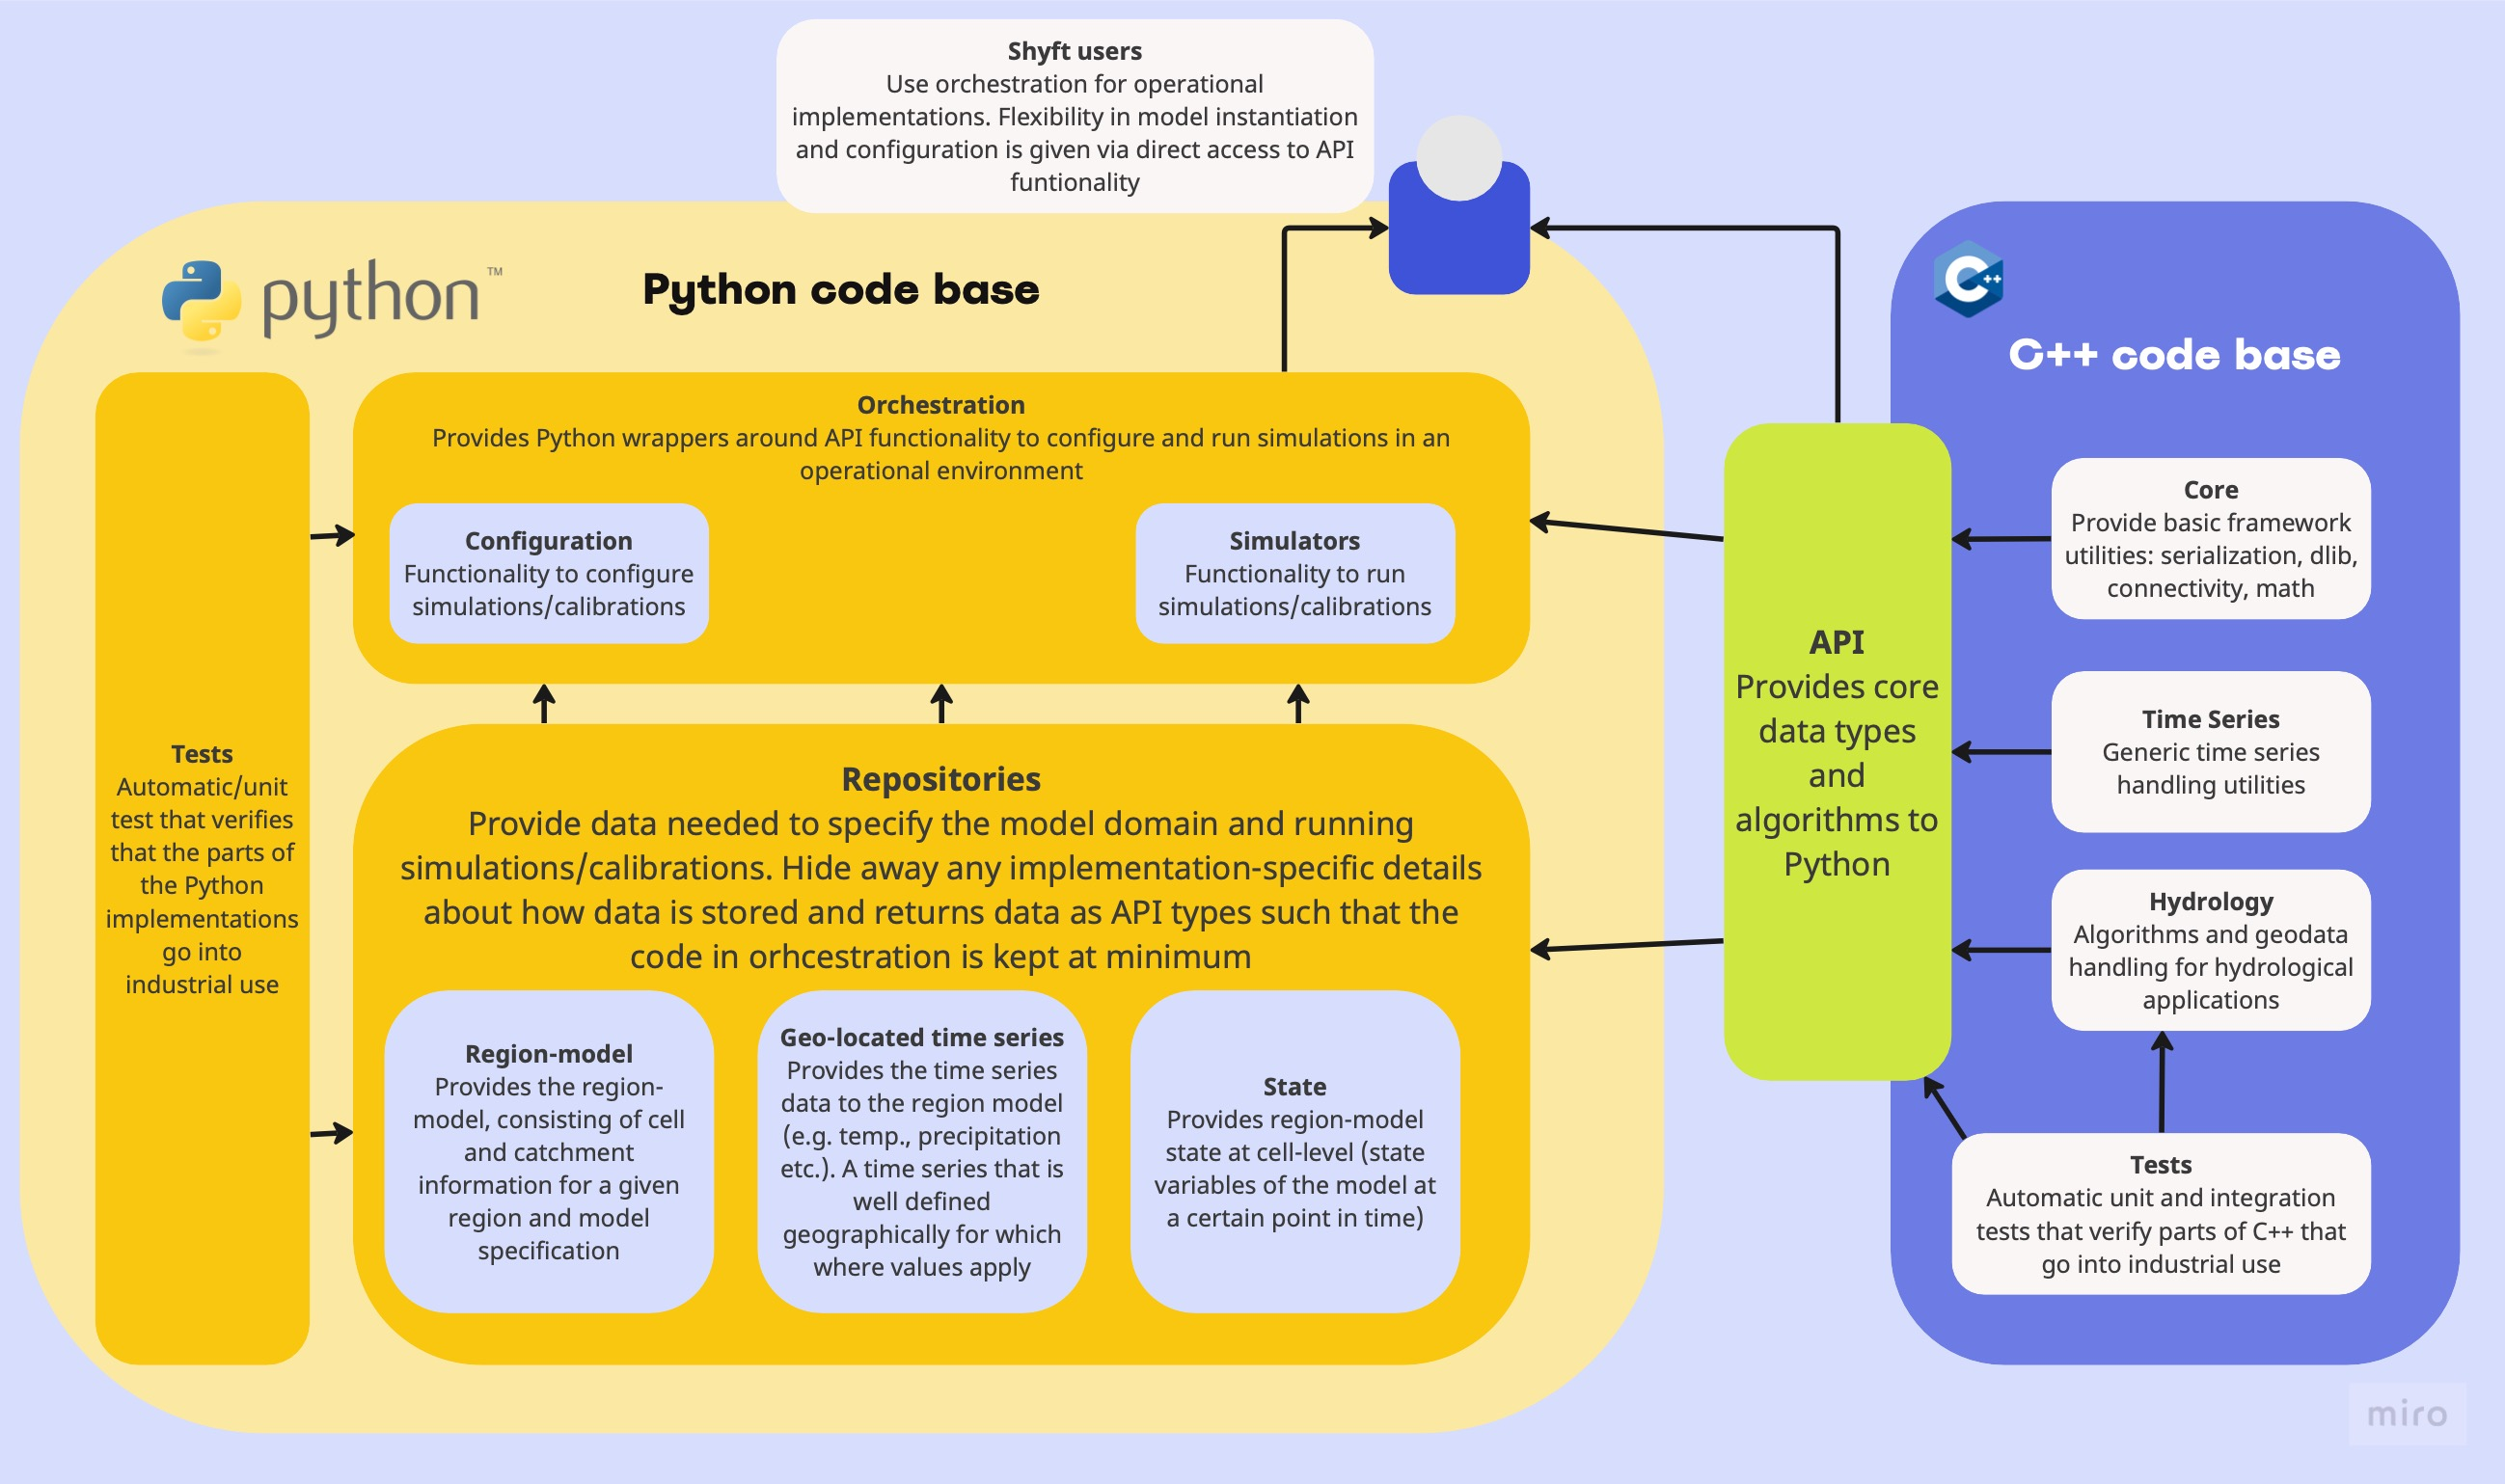
\includegraphics[width=1.1\textwidth,height=11cm]{figures/methods/Shyft Architecture.jpg}
    \caption{Shyft arcitechture. The figure is an adaptation of the figure in \autocite{burkhartShyftV4Framework2021}, and was made using \href{https://miro.com}{Miro}.}
    \label{fig:shyft_architecture}
\end{figure}


\begin{figure}[ht]
    \centering
    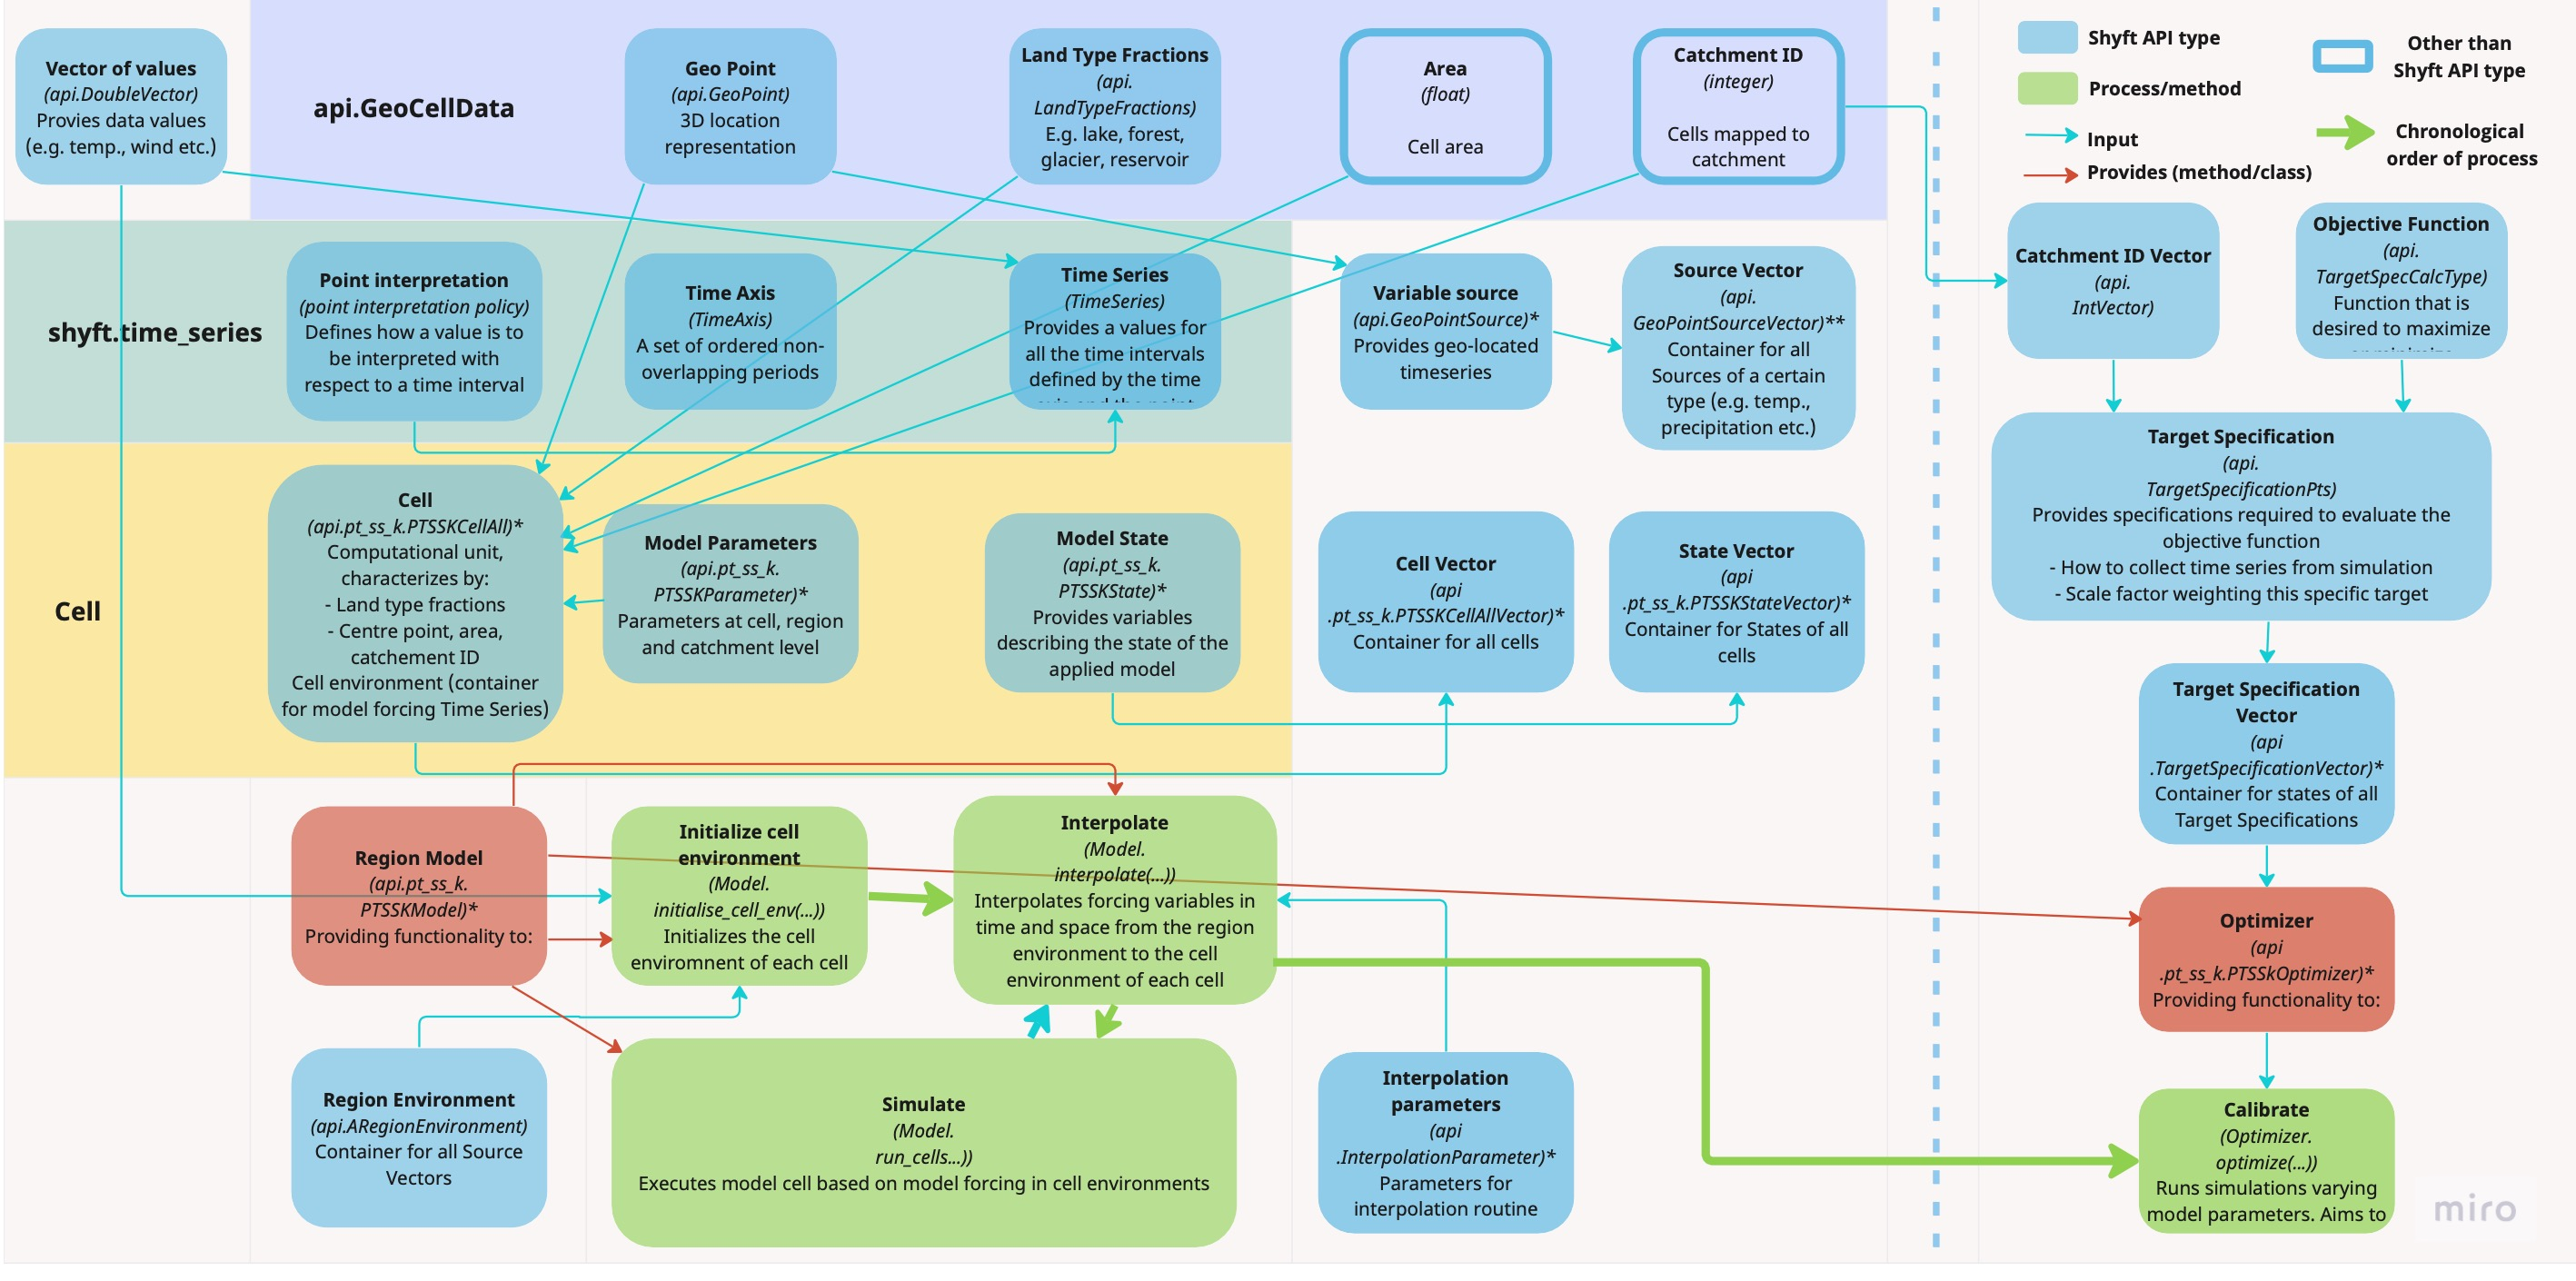
\includegraphics[width=1.1\textwidth,height=13cm]{figures/methods/Swimlane Diagram.jpg}
    \caption{Overview of the main Shyft API types. API types used for simulation are shown to the left of the blue dashed line, while calibration API types are found to the right of the blue dashed line. The figure shows an example of the PTSSK model stack (Priestly-Taylor-Skaugen-Snow-Kirchner). The figure is an adaptation of the figure in \autocite{burkhartShyftV4Framework2021}, and was made using \href{https://miro.com}{Miro}.}
    \label{fig:shyft_api_types}
\end{figure}

\subsubsection{C++ core}
The C++ code base contains several separate code folders \autocite{burkhartShyftV4Framework2021}. The core folder handles framework-related functionality such as serialization; the hydrology folder includes hydrological algorithms and the time series folder handles generic time series. 

\subsubsection{Python API}

The Shyft API is providing the relevant Shyft Core implementations that are needed to configure and utilize models in Python \autocite{burkhartShyftV4Framework2021}. \autoref{fig:shyft_api_types} gives an overview of the main Shyft API types. The idea behind the Python API is that users can write pure Python code without being exposed to the C++ code base. The API allows the user to configure and run a model and access data at various levels. Once a model is initiated, the data is stored at a random access memory of the computer, and the user can access the data using interactive shell commands like Jupyter Notebook or IPython. Thus, the Shyft API allows the user to interactively configure the model, provide forcing data to it, run the model, extract and plot variables. Model parameters can easily be updated once the model is instantiated in this way.

$shyft.time\_series$ is an API type that provides mathematical and statistical operations and functionality for time series \autocite{burkhartShyftV4Framework2021}. Time series can be either expressions or concrete time series. Expressions are time series that are defined by a mathematical expression, while concrete time series are time series that are defined by a set of points in time. All time series have a time axis (set of non-overlapping periods), values and a point interpretation policy. The point interpretation policy defines how the value of a time series is interpreted at a given point in time, and can be either instant value, average value or sum value. 

$api.GeoCellData$ represents common constant cell properties, regardless of model and cell assemblies. The GeoCellData object contains the following properties: elevation, latitude, longitude, slope, aspect, land type, soil type, land cover fraction, soil moisture, snow cover fraction, and the cell area.

$Cell$ contains $GeoCellData$ and $TimeSeries$ of model forcings ($api.GeoPointSource$) \autocite{burkhartShyftV4Framework2021}. The $Cell$ is also specific to the $Model$ selected. The $CellVector$ is a container for all the cells. 

$RegionModel$ is a container for all the $Cells$ and the $Model Parameters$ at region and catchment level. Since everything is vectorized, the $Model State$ collects all the states for each cell \autocite{burkhartShyftV4Framework2021}. The region model provides functionality like: initialization ($Model.initialize\_cell\_env(...)$), interpolation ($Model.interpolate(...)$), simulation ($Model.run\_cells()$), calibration ($Optimizer.optimize(...)$). The $GoalFunction$ that is being minimized is based upon the $TargetSpecification$ in the optimizer.

$Region environment$ contains all the $Source$ vectors of a certain type (e.g. precipitation, temperature, etc.) \autocite{burkhartShyftV4Framework2021}. 

\subsubsection{Repositories}

The necessary data for running simulations depends on the chosen hydrological model. At a minimum, most models requires temperature and precipitation, but some models also require wind speed, relative humidity and shortwave radiation. 

The data required to run simulations in Shyft are managed through repositories \autocite{fowlerPatternsEnterpriseApplication2003}. A repository is a Python based interface to data \autocite{masnunInterfacesPythonProtocols}. Each repository in Shyft has a specific function, a defined interface and multiple implementations of these interfaces. The repositories return data in Shyft API types in order to keep the code in Shyft orchestration at a minimum. The following interfaces are available in Shyft:

\begin{quote}
    \textbf{\textit{Region model repository}:} Presents a configured region model, without revealing underlying implementation specific details regarding the storage of model configuration and data (such as netCDF files).

    \textbf{\textit{Geo-located time series repository}:} Provides geo-located time series for for meteorology- and hydrology-relevant types.

    \textbf{\textit{Interpolation parameter repository}:} Gives parameters for the interpolation method utilized in the simulation.

    \textbf{\textit{State repository}:} Stores the model states and provides them to the region model.

\end{quote}

\subsection{Orchestration}

The orchestration layer is the composition of the simulation configuration \autocite{burkhartShyftV4Framework2021}. This includes defining the model domain, selecting datasets and model algorithms, and presenting the results. The Shyft orchestration is built on top of the API functionalities and offers utilities for configuring, running and post-processing of simulation. The two main objectives of the orchestration are to offer easy entry points for users of Shyft and to utilize all the functionalities of Shyft in operational environments.


The primary model forcing variables in Shyft are precipitation, atmospheric temperature, wind speed, shortwave radiation and relative humidity. 


\begin{table}[ht]
\centering
\caption{Forcing data and validation data}
\label{tab:forcing_validation}
\begin{tabular}{llll}
\toprule
\textbf{Input}    & \textbf{Units}   & \textbf{Source} & \textbf{Temporal resolution} \\
\hline
\multicolumn{4}{l}{\textit{Input for model simulations in Shyft}}                     \\
\hline
Precipitation     & mm h$^{-1}$      & WFDE5           & Hourly                       \\
Temperature       & $^{\circ}$C      & WFDE5           & Hourly                       \\
Wind speed        & m s$^{-1}$       & WFDE5           & Hourly                       \\
Relative humidity & -                & WFDE5           & Hourly                       \\
Global radiation  & W m$^{-2}$       & WFDE5           & Hourly                       \\
\hline
\multicolumn{4}{l}{\textit{Data used for validation}}                                 \\
\hline
Discharge         & m$^{3}$ s$^{-1}$ & DHM             & Hourly                       \\
Snow cover        & per pixel        & MODIS           & 8-day    \\
\bottomrule
\end{tabular}%
\end{table}


\subsection{Spatial interpolation}




\subsection{Hydrological model}





\begin{figure}[ht]
    \centering
    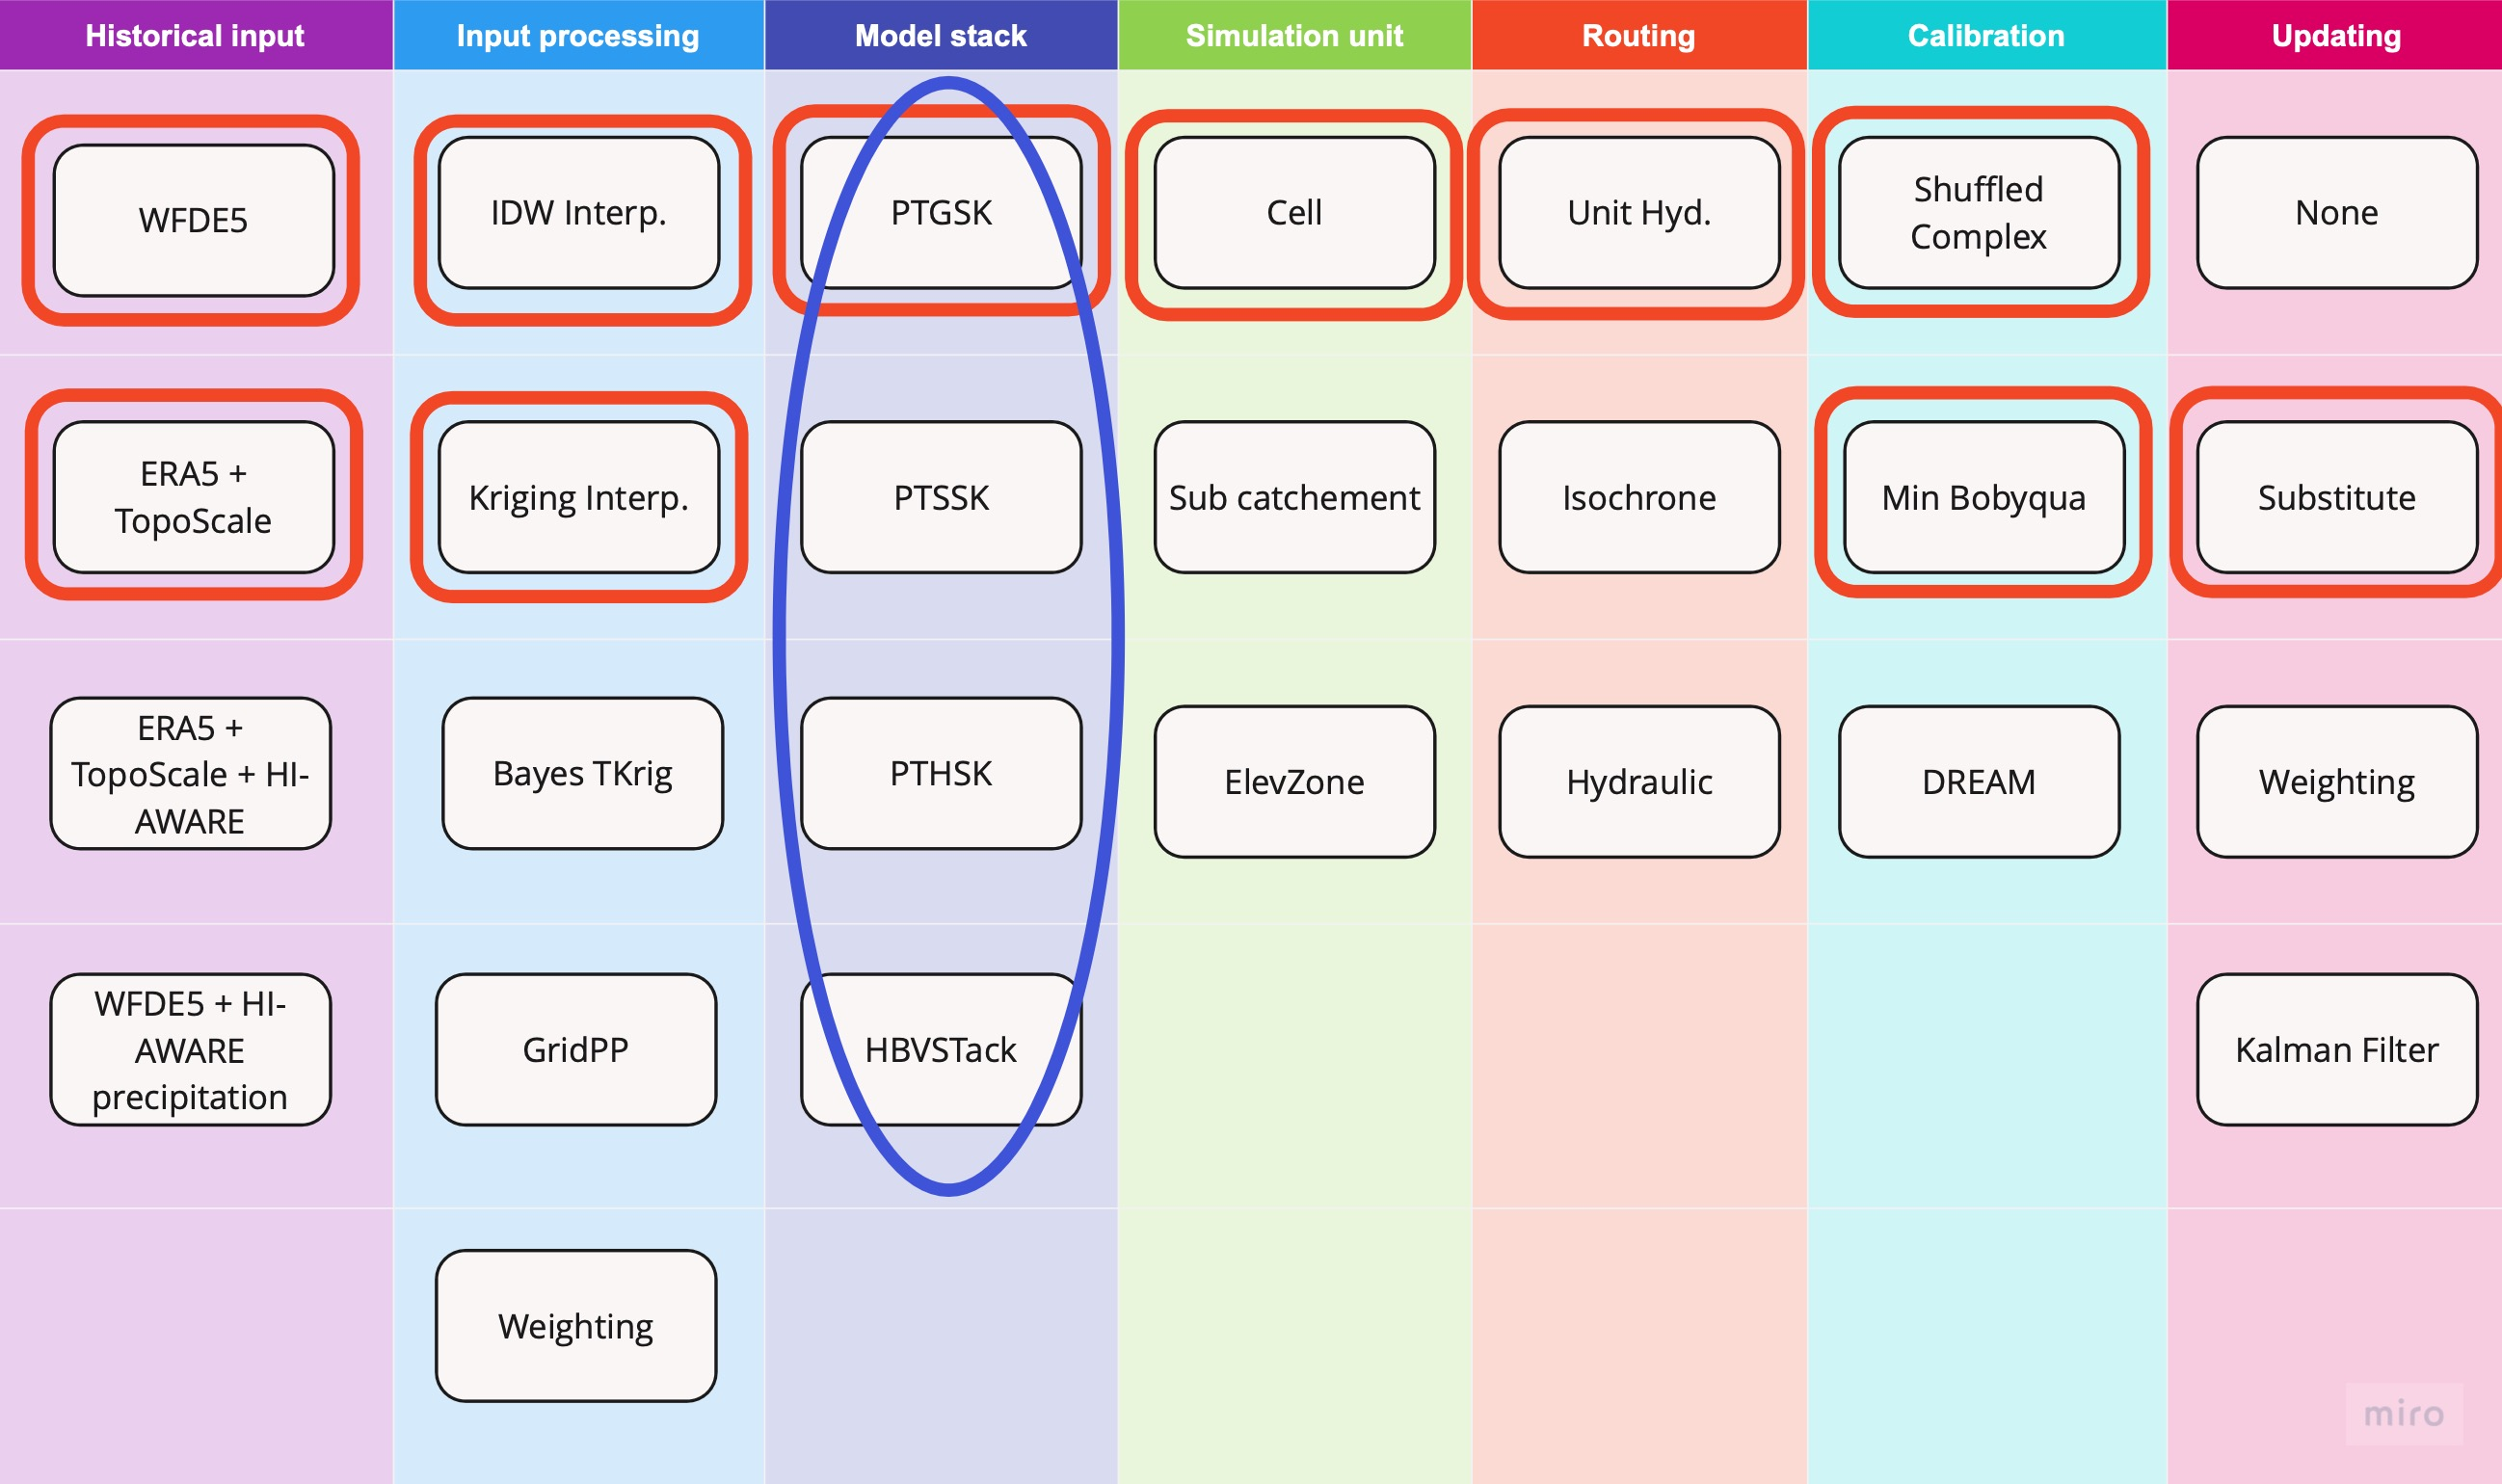
\includegraphics[width=1.1\textwidth,height=10cm]{figures/methods/configs-4.jpg}
    \caption{Evalutation of multiple configurations. The figure is made using \href{https://miro.com}{Miro}, and it is an adaptation of the figure in \autocite{burkhartShyftV4Framework2021}}
    \label{fig:configurations}
\end{figure}

\begin{figure}[ht]
    \centering
    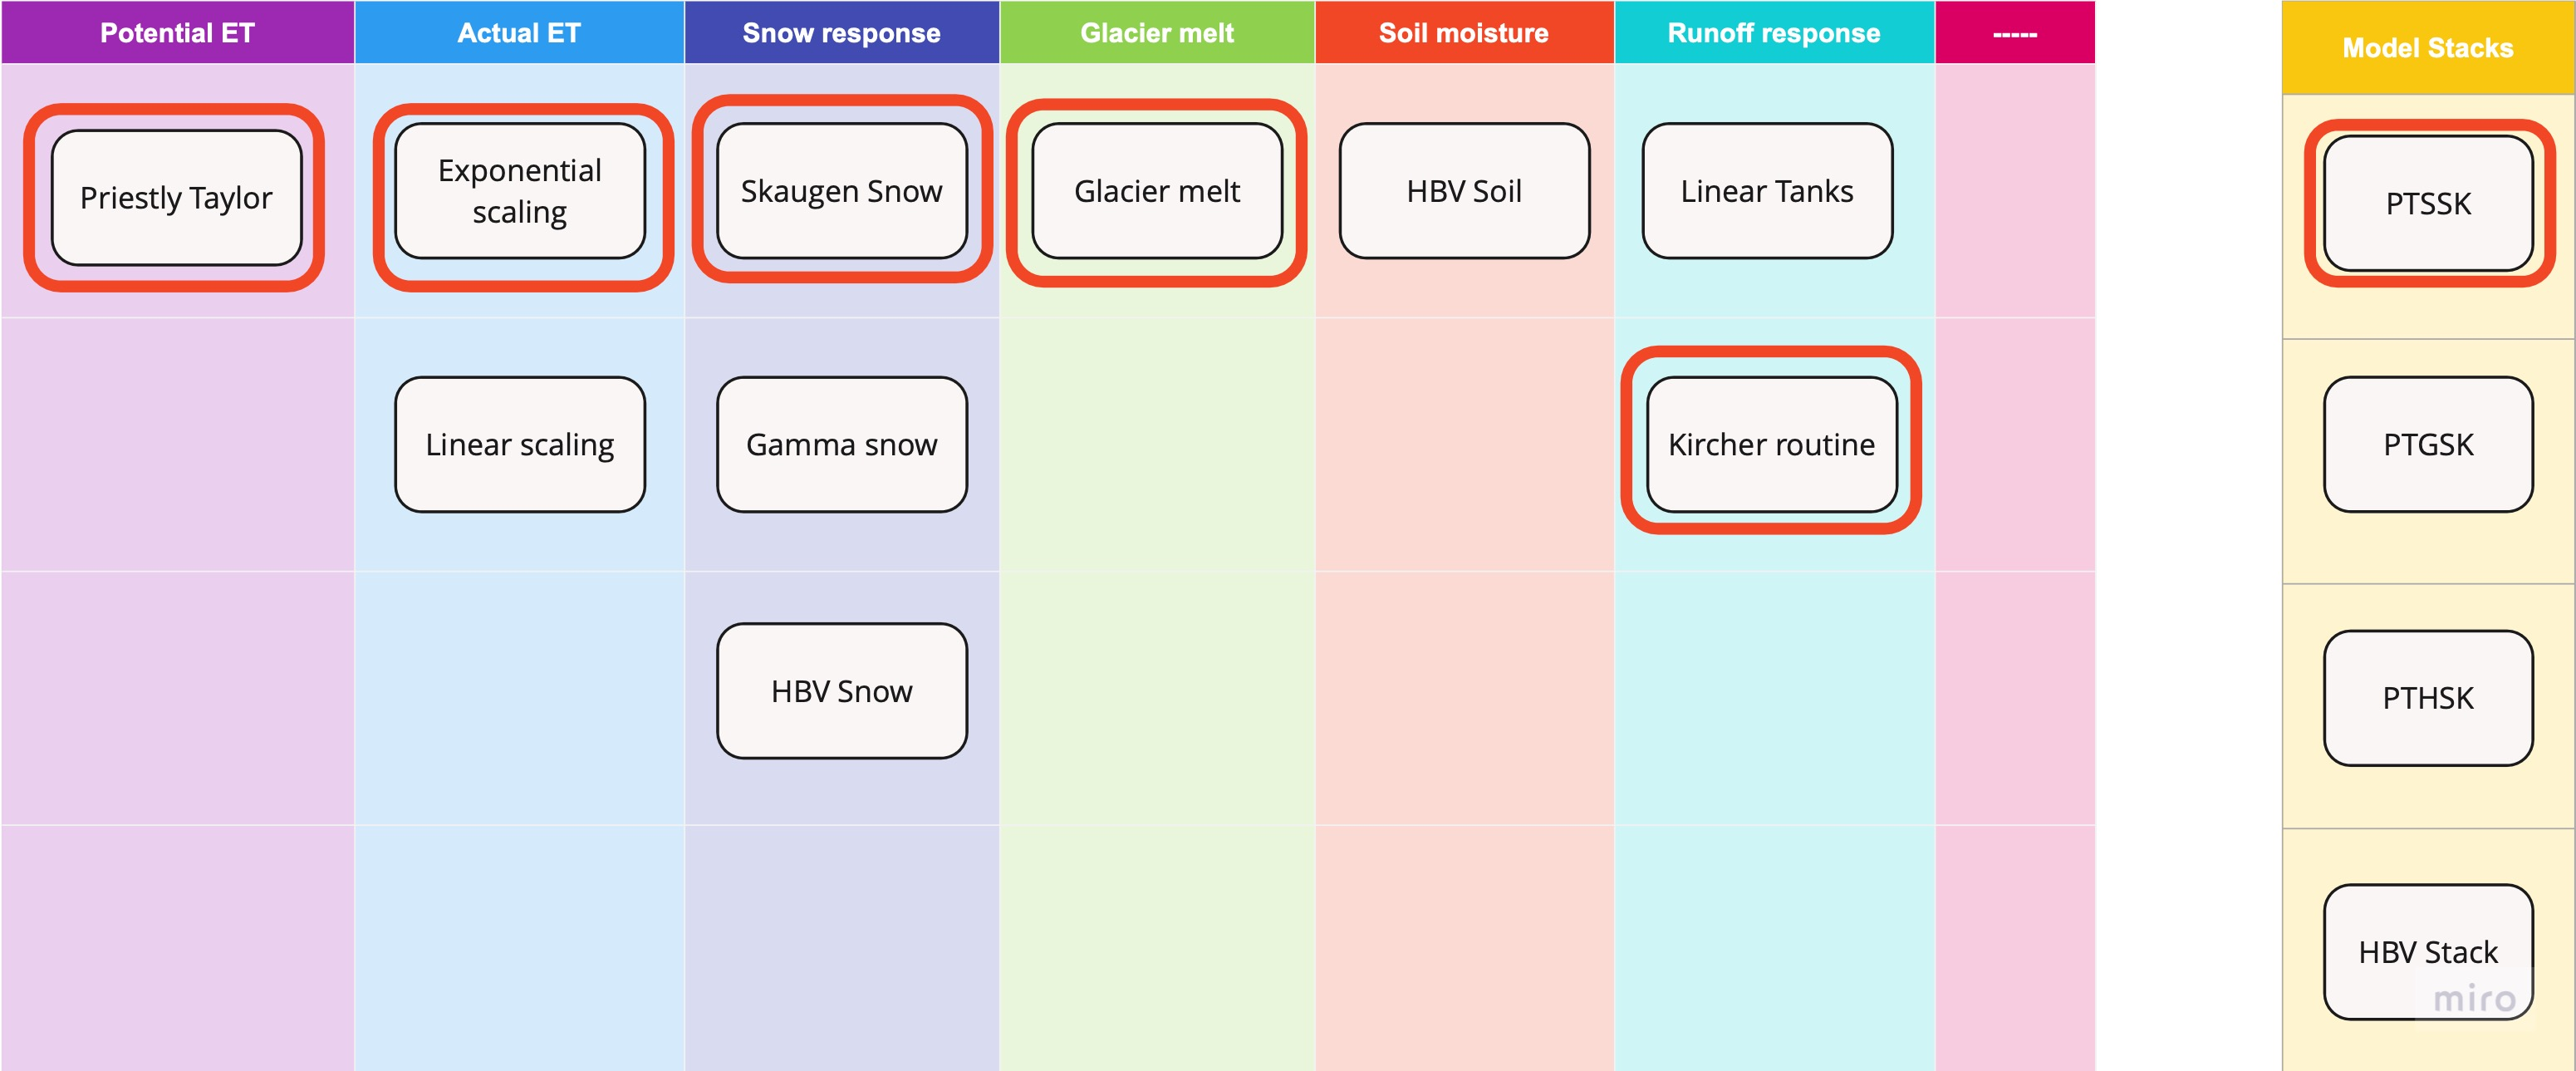
\includegraphics[width=1.1\textwidth,height=8cm]{figures/methods/configs.jpg}
    \caption{Model Stacks components. The figure is made using \href{https://miro.com}{Miro}, and it is an adaptation of the figure in \autocite{burkhartShyftV4Framework2021}}
    \label{fig:model_stack}
\end{figure}


\subsection{Model simulation}



\subsection{Model calibration}

% Please add the following required packages to your document preamble:
% \usepackage[table,xcdraw]{xcolor}
% If you use beamer only pass "xcolor=table" option, i.e. \documentclass[xcolor=table]{beamer}
\begin{table}[ht]
\centering
\caption{Model calibration parameters}
\label{tab:cali_parms}
\begin{tabular}{llllll}
&
  \textbf{Description} &
  \textbf{Parameter used} &
  \textbf{Lower} &
  \textbf{Upper} &
    \\ 
\textbf{Parameter} &
  \textbf{and unit} &
  \textbf{in the submodel} &
  \textbf{limit} &
  \textbf{limit} &
  \textbf{Sources} \\ \toprule
& Outlet & & & &  \\
$c_1$             & empirical coeff. 1 (–) & K  & -8.0  & 0.0   & \autocite{lombranaEvaluationsSnowSimulations2017,sapkotaRegionalModellingNarayani2016} \\
& Outlet & & & &  \\
$c_2$             & empirical coeff. 2 (–) & K  & -1.0  & 1.2   & \autocite{lombranaEvaluationsSnowSimulations2017,sapkotaRegionalModellingNarayani2016}  \\
& Outlet & & & &  \\
$c_3$             & empirical coeff. 3 (–) & K  & -0.15 & -0.05 & \autocite{lombranaEvaluationsSnowSimulations2017,sapkotaRegionalModellingNarayani2016}  \\
\multicolumn{6}{l}{\textbf{Prescribed parameters}}                             \\ \hline
$ae$ scale factor & Scaling factor for AE (–)          & AE & 1.0   & 1.0   & \autocite{lombranaEvaluationsSnowSimulations2017,sapkotaRegionalModellingNarayani2016} \\ 
\bottomrule

\multicolumn{6}{l}{'K' is the catchment response function and 'AE' is actual evapotranspiration.}   \\      
\end{tabular}
\end{table}

\subsection{Water balance estimation}

\subsection{Model validation}

\subsection{Model performance evaluation}